\documentclass[11pt,a4paper]{article}
\usepackage[T1]{fontenc}\usepackage{lmodern}
\usepackage[margin=22mm,headheight=14pt]{geometry}
\usepackage{amsmath,amssymb,bm,booktabs,tabularx,array,graphicx,float,fancyhdr,microtype,xcolor}
\usepackage[colorlinks=true,linkcolor=blue!45!black,urlcolor=blue!45!black,citecolor=blue!45!black]{hyperref}
\setlength{\parindent}{0pt}\setlength{\parskip}{5pt}\renewcommand{\arraystretch}{1.15}
\pagestyle{fancy}\fancyhf{}\fancyhead[L]{\small QFT Project B | Step 7}\fancyhead[R]{\small Group B}\fancyfoot[C]{\thepage}
\newcommand{\dd}{\mathrm{d}}
\begin{document}\hypersetup{pageanchor=false}
\begin{titlepage}\centering\vspace*{3mm}

\includegraphics[width=36mm]{assets/bits_logo.png}\par\vspace{13mm}
{\Large\bfseries BITS PILANI K.K. BIRLA GOA CAMPUS\par}\vspace{3mm}
{\large\bfseries Department of Physics\par}\vspace{18mm}
{\LARGE\bfseries What Quantum Trace Can\\[2mm] a Heavy Particle Leave?\par}\vspace{6mm}
{\large Curvature--Spectator Entanglement\\and the Cosmological Collider\par}\vspace{10mm}
{\large\bfseries Step 7: Spectator Bispectrum\par}\vspace{17mm}
{\Large\bfseries Group-B\par}\vspace{5mm}
\begin{tabular}{ll}Priyansh Rawat & 2023B5A70968G\\Mayank Sinha & 2023B5A70942G\\Samarth Bhatnagar & 2023B5A70853G\end{tabular}
\vfill{\large Under Professor: Rudranil Basu\par}\vspace{7mm}{29 October 2026\par}
\end{titlepage}\setcounter{page}{1}\hypersetup{pageanchor=true}
\section{Mixed contractions and the spectator three-point function}
We use $H_I=\lambda_3\int\dd^3x\,a^4\sigma^3/3!$, with $\lambda_3/H=0.01$. The cubic interaction is treated to first order about the stable quadratic state. Define
\begin{equation}K_k(\eta_f,\eta)=\sum_{a=1}^2q_k^a(\eta_f)\sigma_k^{a*}(\eta).\end{equation}
Wick's six contractions cancel $3!$. If $\langle OH_I\rangle$ contains the product $K_1K_2K_3$, reversing the operator order gives its complex conjugate. Consequently, $-i(Z-Z^*)=2\operatorname{Im}Z$, and
\begin{equation}B_q(k_1,k_2,k_3)=2\lambda_3\int\dd\eta\,a^4\operatorname{Im}(K_{k_1}K_{k_2}K_{k_3}).\end{equation}
For $(k_1,k_2,k_3)=(r,1,1)$ and $z=-k_S\eta$, all legs share the final physical time. The short argument is $z_f$ and the long argument is $rz_f$. A final long-leg value at $z_f$ would evaluate a different physical time.
Let $C_S(z)=\sum Q_a(z_f)\Sigma_a^*(z)$ and $C_L(z)=\sum Q_a(rz_f)\Sigma_a^*(rz)$. With $H=k_S=1$,
\begin{equation}F(r)=\frac{HB_q}{P_q(r)P_q(1)}=\frac{2\lambda_3}{p_Lp_S}\int_{z_f}^{\infty}\frac{\dd z}{z^4}\operatorname{Im}[C_L(z)C_S^2(z)],\end{equation}
where $p_L=\sum|Q_a(rz_f)|^2$ and $p_S=\sum|Q_a(z_f)|^2$. The $r^{-3}$ factors cancel. Power spectra alone cannot replace these complex contractions.

\newpage
\section{Regulated pilot and control tests}
The pilot uses $M=2$, $g=0.1$, $z_f=0.01$, $X=800$ and the sixth-order ultraviolet initial state. The displayed cumulative integral includes $e^{-0.025(2+r)z}$ and stops at $z_{\max}=320$. These finite-regulator values are inputs to Step 8, rather than the final extrapolation.
\begin{figure}[H]\centering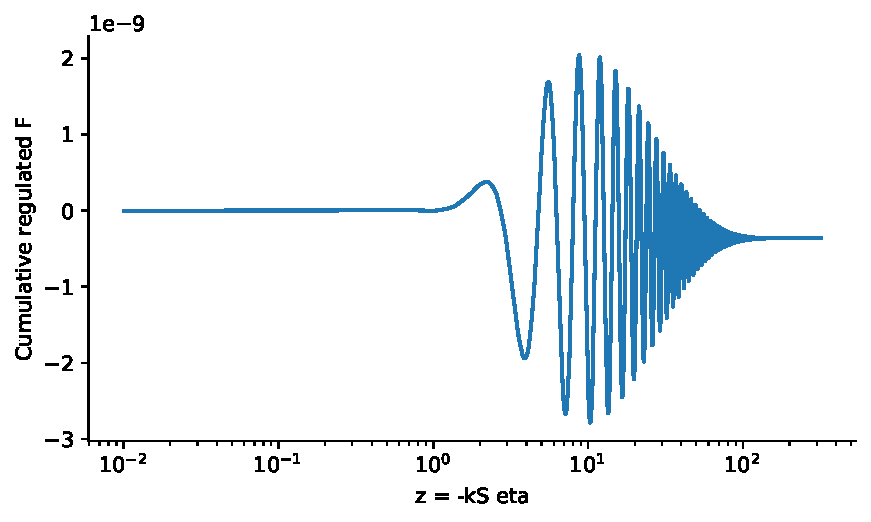
\includegraphics[width=.91\linewidth]{figures/cumulative_integral.pdf}\caption{Cumulative regulated bispectrum for $r=0.03$. Keeping its time dependence makes cancellations and an unfinished early-time remainder visible.}\end{figure}The calculation returns exactly zero for $g=0$ and for $\lambda_3=0$. Doubling $\lambda_3$ doubles the result. The weak-mixing table compares $g=0.025,0.05,0.1$ through $F/g^3$, testing the expected leading cubic mixing scaling.
The saved complex mode file contains the rows $(Q,\Pi_q,\Sigma,\Pi_\sigma)$, two mode columns and an oscillation-resolving early-time grid. The integrand archive stores complex integrand values, quadrature nodes and weights, final powers and settings. These are retained because a single final number cannot independently expose a phase or cancellation error.\begin{thebibliography}{9}\small
\bibitem{chen} X. Chen and Y. Wang, \emph{Quasi-Single Field Inflation and Non-Gaussianities}, JCAP 04 (2010) 027, \href{https://arxiv.org/abs/0911.3380}{arXiv:0911.3380}.
\bibitem{collider} N. Arkani-Hamed and J. Maldacena, \emph{Cosmological Collider Physics}, \href{https://arxiv.org/abs/1503.08043}{arXiv:1503.08043}.\end{thebibliography}
\textbf{Code and supporting data:} \href{https://github.com/rawatpriyansh17/QFT-PROJECT-GROUP-B/tree/main/step7}{step7 on GitHub}.\newpage\section*{Contributions (equal)}\begin{center}\begin{tabularx}{\linewidth}{p{33mm}X}\toprule Member & Contribution\\\midrule Priyansh Rawat & Mixed-contraction and bispectrum derivation.\\[3mm]Samarth Bhatnagar & Common-final-time and zero/cubic controls.\\[3mm]Mayank Sinha & Complex-mode integration, saved phases and figures.\\\bottomrule\end{tabularx}\end{center}\end{document}